\subsection{Results}

Transforming rewards rather than Q-values yielded less positive results than \tloA{} (Figure~\ref{fig:online_performance_exp2}). SFELLA continued to improve on \tloA{} under some circumstances in the UnbreakableBottles environment, but SFELLA did not outperform \tloA{} in BreakableBottles as it did in Experiment 1. 

\begin{figure}
  %\centering
  %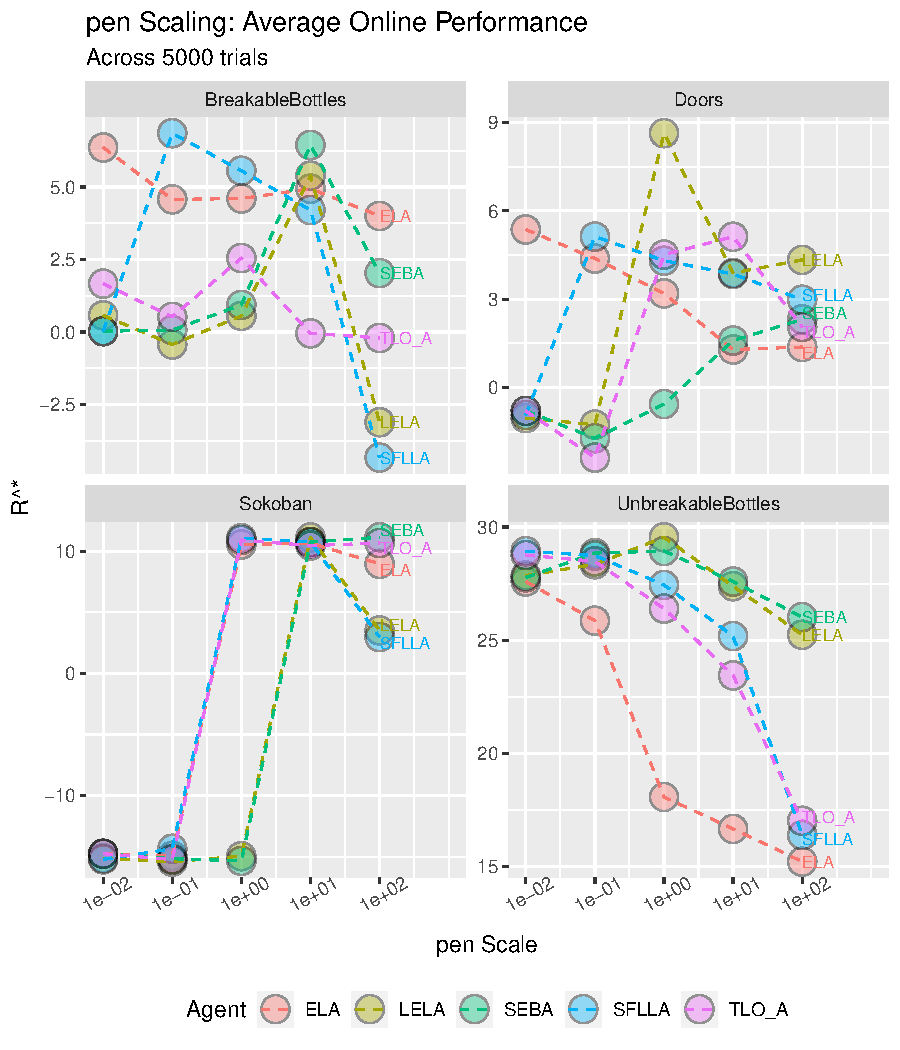
\includegraphics[width=\columnwidth]{output/onlinepen.pdf}
  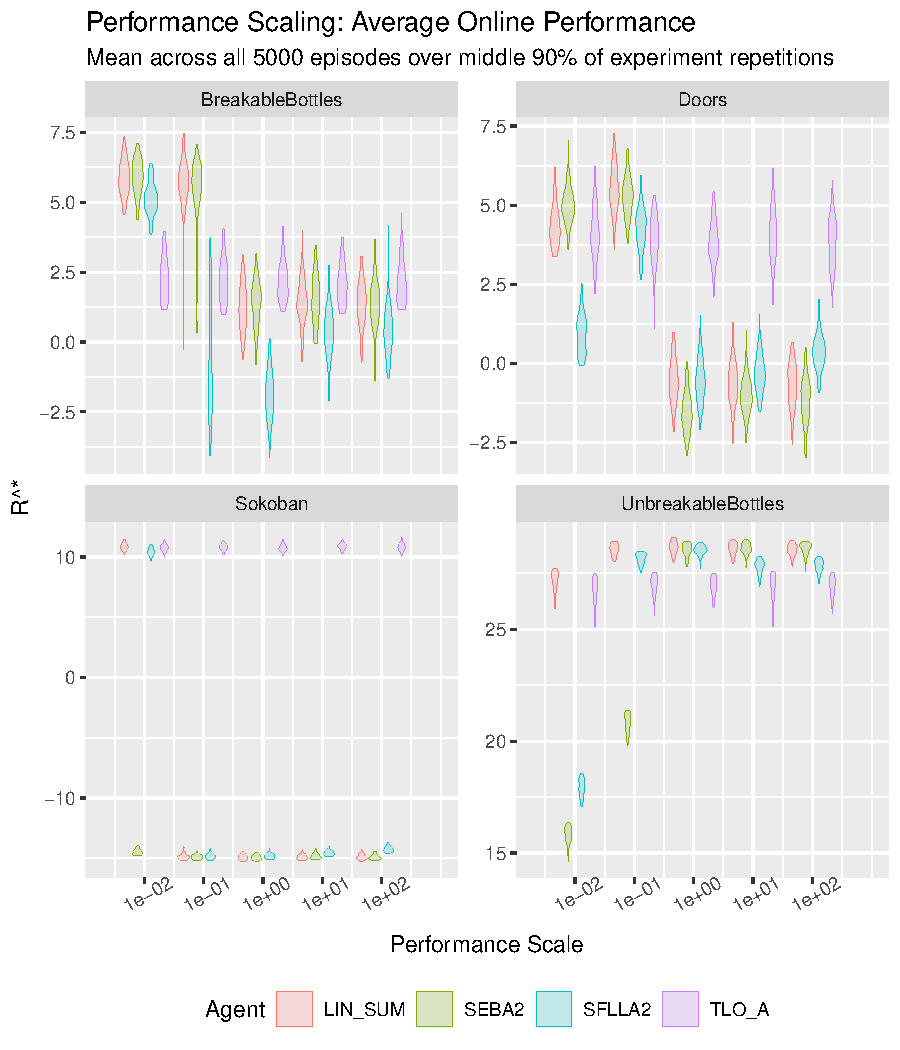
\includegraphics[width=\columnwidth]{output/multirun_n100_reward_to_util_transformonline_util_transform_Performance.pdf}
  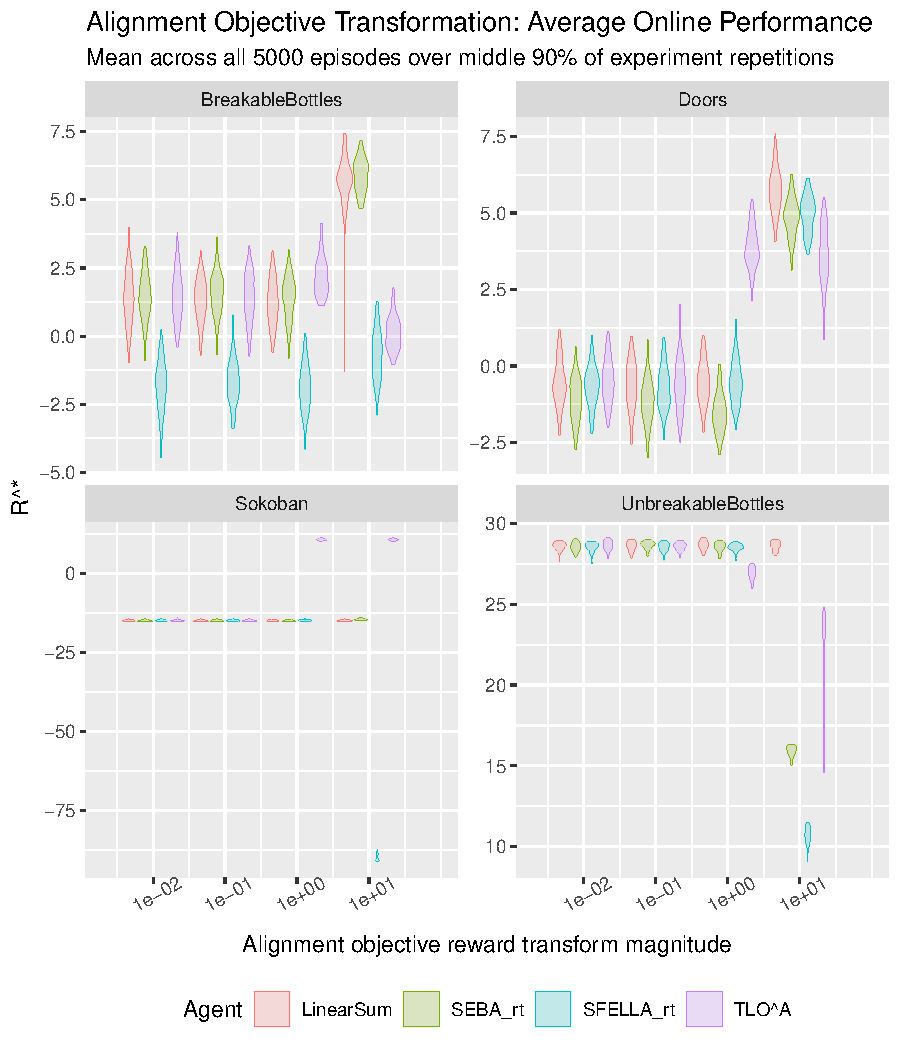
\includegraphics[width=\columnwidth]{output/multirun_n100_reward_to_util_transformonline_util_transform_Alignment.pdf}
  \caption{Experiment 2: \RStar{} Online performance across learning episodes and experiment repetitions for different reward transformations. In contrast to Q-value transformations as in \ref{fig:online_performance}, when reward is transformed, SFELLA no longer performs better than \tloA{} in the BreakableBottles environment, and SFELLA performs much worse than \tloA{} in the Doors environment.
  }
   \label{fig:online_performance_exp2}
 \end{figure}